% Paquets généraux
\documentclass[a4paper,12pt,titlepage]{article}
\usepackage[T1]{fontenc}
\usepackage[utf8]{inputenc}
\usepackage[french]{babel}
\usepackage[gen]{eurosym}
%\usepackage[dvips]{graphicx}
\usepackage{fancyhdr}
\usepackage{pdfpages} 
\usepackage{multido}
\usepackage{moreverb}
\usepackage{hyperref}
%\usepackage{textcomp}
\usepackage{verbatim}
\usepackage{moreverb}
\usepackage{listings}
\usepackage{minted}
\usepackage{eso-pic}
\usepackage{enumitem}
\usepackage{comment}
\usepackage{boxedminipage}
\usepackage[french,onelanguage, boxruled,linesnumbered]{algorithm2e}


\newcommand{\auteurun}{Juliette Genzmer}
\newcommand{\auteurdeux}{Willie Robert}
\newcommand{\auteurtrois}{Renaud Costadoat}
\newcommand{\institute}{Lycée Dorian}
\newtheorem{solution}{Solution}


\newcommand{\nom}{Porte conteneur}
\newcommand{\sequence}{03}
\newcommand{\num}{04}
\newcommand{\type}{TD}
\newcommand{\descrip}{Résolution d'un problème en utilisant des méthodes algorithmiques}
\newcommand{\competences}{Alt-C3: Concevoir un algorithme répondant à un problème précisément posé}

\usepackage{color}
\usepackage{xcolor}
\usepackage{colortbl}
\usepackage{helvet}
\renewcommand{\familydefault}{\sfdefault}
\usepackage{amsfonts}
\usepackage{amsmath}
%\usepackage{xspace}
\usepackage{varioref}
\usepackage{tabularx}
%\usepackage{floatflt}
\usepackage{graphics}
\usepackage{wrapfig}
\usepackage{textcomp}
\usepackage{tikz}
\usepackage{wrapfig}
\usepackage{gensymb}
\usepackage{ifthen}
\usepackage{cancel}
\usepackage{etoolbox}
\usepackage{multirow}
%\usepackage{boxedminipage}
\definecolor{gris25}{gray}{0.75}
\definecolor{bleu}{RGB}{18,33,98}
\definecolor{bleuf}{RGB}{42,94,171}
\definecolor{bleuc}{RGB}{231,239,247}
\definecolor{rougef}{RGB}{185,18,27}
\definecolor{rougec}{RGB}{255,188,204}%255,230,231
\definecolor{vertf}{RGB}{103,126,82}
\definecolor{vertc}{RGB}{220,255,191}
\definecolor{forestgreen}{rgb}{0.13,0.54,0.13}
\definecolor{blcr}{rgb}{0.59,0.69,0.84}
\definecolor{blfr}{rgb}{0.32,0.51,0.75}
\definecolor{orfr}{rgb}{0.90,0.42,0.15}
\definecolor{orcr}{rgb}{0.90,0.65,0.50}
\definecolor{orangef}{rgb}{0.659,0.269,0.072}
\definecolor{orange}{rgb}{0.58,0.35,0.063}
\definecolor{orangec}{rgb}{0.43,0.32,0.25}
\definecolor{rcorrect}{rgb}{0.6,0,0}
\definecolor{sequence}{rgb}{0.75,0.75,0.75}
\definecolor{competences}{rgb}{0.61,0.73,0.35}
\definecolor{grisf}{HTML}{222222}
\definecolor{grisc}{HTML}{636363}
\definecolor{normal}{HTML}{4087c4}
\definecolor{info}{HTML}{5bc0de}
\definecolor{success}{RGB}{92,184,92}
\definecolor{warning}{RGB}{240,173,78}
\definecolor{danger}{RGB}{217,83,79}
\hypersetup{                    % parametrage des hyperliens
    colorlinks=true,                % colorise les liens
    breaklinks=true,                % permet les retours à la ligne pour les liens trop longs
    urlcolor= blfr,                 % couleur des hyperliens
    linkcolor= orange,                % couleur des liens internes aux documents (index, figures, tableaux, equations,...)
    citecolor= forestgreen                % couleur des liens vers les references bibliographiques
    }

% Mise en page
\pagestyle{fancy}

\setlength{\hoffset}{-18pt}

\setlength{\oddsidemargin}{0pt} 	% Marge gauche sur pages impaires
\setlength{\evensidemargin}{0pt} 	% Marge gauche sur pages paires
\setlength{\marginparwidth}{00pt} 	% Largeur de note dans la marge
\setlength{\headwidth}{481pt} 	 	% Largeur de la zone de tête (17cm)
\setlength{\textwidth}{481pt} 	 	% Largeur de la zone de texte (17cm)
\setlength{\voffset}{-18pt} 		% Bon pour DOS
\setlength{\marginparsep}{7pt}	 	% Séparation de la marge
\setlength{\topmargin}{-30pt} 		% Pas de marge en haut
\setlength{\headheight}{55pt} 		% Haut de page
\setlength{\headsep}{20pt} 		% Entre le haut de page et le texte
\setlength{\footskip}{30pt} 		% Bas de page + séparation
\setlength{\textheight}{700pt} 		% Hauteur de l'icone zone de texte (25cm)
\setlength\fboxrule{1 pt}
\renewcommand{\baselinestretch}{1}
\setcounter{tocdepth}{1}
\newcommand{\cadre}[2]
{\fbox{
  \begin{minipage}{#1\linewidth}
   \begin{center}
    #2\\
   \end{center}
  \end{minipage}
 }
}

\newcounter{num_quest} \setcounter{num_quest}{0}
\newcounter{num_rep} \setcounter{num_rep}{0}
\newcounter{num_cor} \setcounter{num_cor}{0}

\newcommand{\question}[1]{\refstepcounter{num_quest}\par
~\ \\ \parbox[t][][t]{0.15\linewidth}{\textbf{Question \arabic{num_quest}}}\parbox[t][][t]{0.85\linewidth}{#1\label{q\the\value{num_quest}}}\par\par
}



\newcommand{\reponse}[0]{\refstepcounter{num_rep}\par
~\ \\ \parbox[t][][t]{0.15\linewidth}{\textbf{Question \arabic{num_rep}}}}

\newcommand{\cor}
{\refstepcounter{num_cor}
\noindent
\rule{\linewidth}{.5pt}
\textbf{Question \arabic{num_cor}:} \\
}



% En tête et pied de page
\lhead{\nom}
\rhead{
\includegraphics[width=2cm]{../../../img/logo}}
\lfoot{David Aubert, Renaud Costadoat}
\rfoot{Page \thepage}
\cfoot{}

\newlength{\RoundedBoxWidth}
\newsavebox{\GrayRoundedBox}
\newenvironment{GrayBox}[1][\dimexpr\textwidth-4.5ex]%
   {\setlength{\RoundedBoxWidth}{\dimexpr#1}
    \begin{lrbox}{\GrayRoundedBox}
       \begin{minipage}{\RoundedBoxWidth}}%
   {   \end{minipage}
    \end{lrbox}
    \begin{center}
    \begin{tikzpicture}%
       \draw node[draw=bleuf,fill=bleuc,rounded corners,%
             inner sep=2ex,text width=\RoundedBoxWidth]%
             {\usebox{\GrayRoundedBox}};
    \end{tikzpicture}
    \end{center}}

\fancypagestyle{correction}{%
  \fancyhf{}
  \lhead{\colorbox{danger}{\begin{minipage}{0.65\paperwidth} \textcolor{white}{\textbf{Correction}} \end{minipage}} }
  \rhead{
\includegraphics[width=2cm]{../../../img/logo}}
  \lfoot{Juliette Genzmer, Willie Robert, Renaud Costadoat}
  \rfoot{\colorbox{danger}{\begin{minipage}{0.3\paperwidth} \begin{flushright}\textcolor{white}{\textbf{Correction}}\end{flushright} \end{minipage}} }}

\renewcommand{\footrulewidth}{0.4pt}


\newcommand{\BackgroundPic}{%
\put(0,0){%
\parbox[b][\paperheight]{\paperwidth}{%
\vfill
\begin{center}
\hspace{0.5cm}\vspace{0.5cm}

\includegraphics[width=\paperwidth,height=\paperheight,%
keepaspectratio]{../../../img/fond5}%
\end{center}
\vfill
}}}

\newcommand{\goforum}{
\begin{figure}[ht!]
\begin{center}
 
\includegraphics[width=0.7\linewidth]{../../../img/go_forum}
\end{center}
\label{go_forum}
\caption{J'pète les plombs}
\end{figure}}

\newcommand{\BackgroundPicdeux}{%
\put(25,-30){%
\parbox[b][\paperheight]{\paperwidth}{%
\vfill
\begin{center}

\includegraphics[width=\paperwidth,height=\paperheight,%
keepaspectratio]{../../../img/fond6}%
\end{center}
\vfill
}}}

\setenumerate[1]{align=left,label=\arabic*}
\setenumerate[2]{before=\stepcounter{enumi},label*=.\arabic*,leftmargin=1.2em,align=left}

\begin{document}


\pagestyle{fancy}

\AddToShipoutPicture{\BackgroundPicdeux}

\begin{center}
{\Large\bf {\type} \no {\numero} -- \descrip}
\end{center}

\SetKw{KwFrom}{de} 

\hspace{-1cm}
\begin{boxedminipage}{\textwidth} 
\begin{itemize}
 \item Faire tous les exercices dans un fichier {NomPrenom.py} à sauvegarder,
 \item mettre en commentaire l'exercice et la question traités (ex: \# Exercice 1),
 \item ne pas oublier pas de commenter ce qui est fait dans votre code (ex: \# Je crée une fonction pour calculer la racine d'un nombre),
 \item il est possible de demander un déblocage pour une question, mais celle-ci sera notée 0,
 \item les deux parties sont indépendantes et peuvent être traitées dans l'ordre que vous voulez,
 \item il faut vérifier avant de partir que le code peut s'exécuter et qu'il affiche les résultats que vous attendez. Les lignes de code qui doivent s'exécuter sont décommentées.
\end{itemize}
\end{boxedminipage}

\section{La décomposition de Zeckendorf}

La suite de Fibonacci $(F_{n})_{n\in \mathbb {N} }$ est définie par $F_{0}=0, F_{1}=1$ et la relation de récurrence $F_{n}=F_{n-1}+F_{n-2}$ pour $n\geq 2$. Le tableau \ref{tab01} donne les 9 premiers termes de la suite de Fibonacci.

\begin{table}[ht!]
\begin{center}
\begin{tabular}{|c|c|c|c|c|c|c|c|c|}
\hline
$F_0$ & $F_1$ & $F_2$ & $F_3$ & $F_4$ & $F_5$ & $F_6$ & $F_7$ & $F_8$\\
\hline
0&1&1&2&3&5&8&13&21 \\
\hline
\end{tabular}
\end{center}
\caption{\label{tab01} 9 premiers termes de la suite de Fibonacci}
\end{table}

\question{On souhaite créer une fonction \verb?fibonacci(n)? qui renvoie l'ensemble des termes de la suite de Fibonacci inférieurs ou égaux à \verb?n?. Compléter le code suivant. Vérifier le résultat grâce à la commande \verb?print(fibonacci(10))? qui doit retourner \verb?[0, 1, 1, 2, 3, 5, 8]?.}

\begin{minted}[linenos]{python}
# -*- coding: utf-8 -*-

def fibonacci(n):
    # valeurs 1 et 0
    if n == 0:
        return [n]        
    elif n == 1:
        return [0,1]
    else:
        f1, f2, f3 = 0, 1, 1
        fibo=[f1,f2,f3]
        while f2+f3 <=n:
            f1 = f2
            f2 = f3
            f3 = f1 + f2
        return fibo

print(fibonacci(10))
\end{minted}

\paragraph{Théorème :} Le théorème de Zeckendorf affirme que tout nombre entier naturel \verb?n? peut s'écrire de manière unique comme une somme de nombres de Fibonacci non nuls et distincts, en imposant la condition que deux nombres consécutifs dans la suite de Fibonacci ne soient pas employés simultanément. 

Il est possible de l'obtenir grâce à l'algorithme glouton suivant:
\begin{algorithm}
\caption{Algorithme de la fonction decomposition\_fibo(n)}\label{alg:two}
\KwData{$n \geq 0$}
\KwResult{$resultat$}
$resultat \gets []$\;
$valeurs \gets fibonacci(n)$\;
$i \gets len(valeurs)-1$\;
\While{$n > 0$}{
  \eIf{$n \geq valeurs[i]$}{
    $resultat \gets valeurs[i]$\;
    $n \gets n-valeurs[i]$\;
    $i \gets i-1$\;
    }
    {}
    $i \gets i-1$\;
}
\end{algorithm}

\question{Coder la fonction \texttt{decomposition\_fibo(n)} à partir de l'algorithme précédent et la tester avec \texttt{print(decomposition\_fibo(14))} qui doit renvoyer \texttt{[13, 1]}.}

\question{Afficher pour chaque entier \texttt{n} de 1 à 22:
\begin{itemize}
 \item la valeur de \texttt{n},
 \item la décomposition de Zeckendorf de \texttt{n}.
\end{itemize}

Vérifier que les conditions du théorème sont respectées pour chaque \verb?n?.}

\section{Le Jeu de la Vie}

Le jeu de la Vie (Game of Life) est un automate cellulaire, devenu un jeu \og\ à zéro joueur\fg\ de simulation mathématique, imaginé par John Horton Conway en 1970. Malgré des règles très simples, il est Turing-complet. 

Le jeu se déroule sur une grille à deux dimensions, théoriquement infinie, dont les cases, appelées \og\ cellules \fg, par analogie avec les cellules vivantes, peuvent prendre deux états distincts : \og vivante \fg\ ou \og\ morte \fg.

Une cellule possède huit voisines, qui sont les cellules adjacentes horizontalement, verticalement et diagonalement.

\newpage

À chaque itération, l'état d’une cellule est entièrement déterminé par l’état de ses huit cellules voisines, selon les règles suivantes :
\begin{itemize}
 \item Une cellule morte possédant exactement \textbf{trois} cellules voisines vivantes devient vivante (elle naît),
 \item Une cellule vivante ne possédant pas exactement \textbf{deux} ou \textbf{trois} cellules voisines vivantes meurt.
\end{itemize}

\subsection{Le cas du blinker}

La configuration 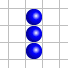
\includegraphics[width=.07\linewidth]{img/Gol-blinker2.png} est suivie par 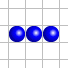
\includegraphics[width=.07\linewidth]{img/Gol-blinker1.png} qui redonne ensuite la première.

\begin{figure}[ht!]
 \begin{minipage}{0.3\linewidth}
 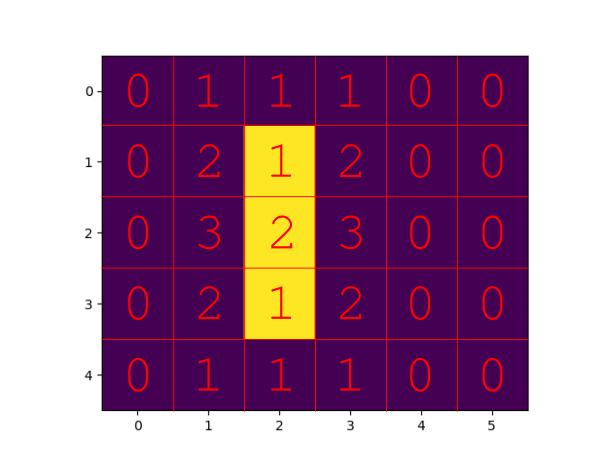
\includegraphics[width=\linewidth]{img/blinker_num}
 \vspace{-1cm}
 \caption{\label{fig01} Blinker}
 \end{minipage}\hfill
 \begin{minipage}{0.68\linewidth}
 \paragraph{Justification} La figure \ref{fig01} présente en clair les cellules vivantes, les autres sont mortes. Le nombre de voisines vivantes a été superposé à la représentation de chaque cellule. Ainsi:
	\begin{itemize}
 		\item les deux cellules mortes ayant 3 voisines vivantes vont s'activer,
		\item celle vivante ayant 2 cellule actives va rester active,
		\item les deux vivantes n'ayant qu'une seule voisine vivante vont mourir.
	\end{itemize}
 \end{minipage}
\end{figure}

Le code suivant permet de tracer la première configuration du blinker et de calculer pour chaque cellule le nombre de cellules voisines vivantes qui l'entourent:
\begin{minted}[linenos]{python}
import numpy as np
import matplotlib.pyplot as plt
from matplotlib.animation import FuncAnimation


M,N=6,5
Z=[[0 for i in range(M)] for i in range(N)]
Z[1][2]=1
Z[2][2]=1
Z[3][2]=1

def calcul_nb_voisins(Z):
    lx,ly = len(Z[0]), len(Z)
    v = [[0] * lx for i in range(ly)]
    for x in range(lx):
        for y in range(ly):
            v[y%ly][x%lx] = Z[(y-1)%ly][(x-1)%lx]+Z[(y-1)%ly][x%lx] \
            +Z[(y-1)%ly][(x+1)%lx] + Z[y%ly][(x-1)%lx] + 0 \
            +Z[y%ly][(x+1)%lx] + Z[(y+1)%ly][(x-1)%lx]\
            +Z[(y+1)%ly][x%lx]+Z[(y+1)%ly][(x+1)%lx]
    return v

print(calcul_nb_voisins(Z))
\end{minted}

\question{Recopier ce code et exécuter ce code. Le vérifier grâce à la commande \texttt{print(calcul\_nb\_voisins(Z))} qui doit renvoyer pour cette configuration :
\begin{center}
[[0, 1, 1, 1, 0, 0],

[0, 2, 1, 2, 0, 0],

[0, 3, 2, 3, 0, 0],

[0, 2, 1, 2, 0, 0],

[0, 1, 1, 1, 0, 0]]
\end{center}}

\textbf{Remarque} : La présence des \verb?%lx? et des \verb?%ly? permet d'éviter les problèmes liés au bordure de la feuille et de simuler le comportement d'un espace infini.

Le code suivant permet de déterminer pour chaque cellule son évolution (\og\ mort\fg\ ou \og\ naissance\fg) en fonction de ses voisines. Il doit être placé à la suite du code précédent.

\begin{minted}[linenos]{python}
def update(frameNum, img, Z):
    lx,ly = len(Z[0]), len(Z)
    N = calcul_nb_voisins(Z)
    for x in range(lx):
        for y in range(ly):
            if Z[y][x] == 1 and  ..................................
                Z[y][x] = 0
            elif Z[y][x] == 0 and  ............................
                Z[y][x] = 1
    img.set_data(Z)
    return img,

fig, ax = plt.subplots()
img = ax.imshow(Z, interpolation='nearest')
ani = FuncAnimation(fig, update, fargs=(img, Z), frames=1000,\
			 interval=1, save_count=1)
plt.show()
\end{minted}

\question{Recopier le code et compléter les lignes 6 et 8 afin d'obtenir le comportement attendu.} 

\newpage

\subsection{Le planeur}

\begin{figure}[ht!]
\begin{minipage}{0.4\linewidth}
\begin{center}
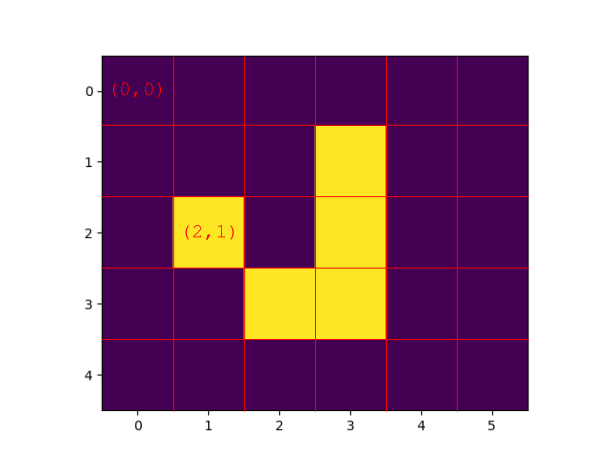
\includegraphics[width=\linewidth]{img/planeur_num}
\end{center}
\caption{\label{fig02}Planeur}
\end{minipage}\hfill
\begin{minipage}{0.55\linewidth}
Une évolution ensuite a été de chercher comment propager la vie. La solution la plus simple pour cela est l'utilisation d'un planeur présenté à la figure \ref{fig02}.
\end{minipage}
\end{figure}

\question{Modifier le code de la question 4 afin de faire apparaître un planeur. Afin de voir son évolution, prendre {M,N=70,50}.}

\subsection{Le canon à planeurs de Gosper}

La dernière forme qui sera présentée dans cette épreuve est le canon à planeurs de Gosper, créé par Bill Gosper. Cette structure émet des planeurs à l'infini.

Comme elle est assez complexe à produire, la matrice \texttt{Z} est fournie dans le fichier \texttt{gosper\_canon.csv} présent dans le dossier de partage.

\question{Ouvrir le fichier 'csv' (séparateur de colonnes ";") et écrire son contenu dans la matrice Z. Puis utiliser le code de la question 6 afin de faire apparaître le canon de Gosper.}

\question{Cette fois-ci le raccordement des bords de la grille pose des problèmes d'affichage, proposer une modification de la fonction \texttt{calcul\_nb\_voisins(Z)} qui permette aux bords de la grille d'arrêter la propagation des cellules.}

\paragraph{Remarque : } Les dernières pages du sujet doivent servir de brouillon.

\finsujet{2}

\reponse{}{
\begin{minted}[linenos]{python}
# -*- coding: utf-8 -*-

def fibonacci(n):
    # valeurs 1 et 0
    if n == 0:
        return [n]        
    elif n == 1:
        return [0,1]
    else:
        f1, f2, f3 = 0, 1, 1
        fibo=[f1,f2,f3]
        while f2+f3 <=n:
            f1 = f2
            f2 = f3
            f3 = f1 + f2
            fibo.append(f3) #il faut ajouter cette ligne
        return fibo

print(fibonacci(10))
\end{minted}
}

\reponse{}{
\begin{minted}[linenos]{python}
def decomposition_fibo(n):
    resultat=[]
    valeurs=fibonacci(n)
    i=len(valeurs)-1
    while n>0:
        if n>=valeurs[i]:
            resultat.append(valeurs[i])
            n = n-valeurs[i]
            i-=1
        i-=1
    return resultat

print(decomposition_fibo(14))
\end{minted}
}


\reponse{}{
\begin{minted}[linenos]{python}
for n in range(23):
    print(n,decomposition_fibo(n))
\end{minted}
}

\reponse{}{Recopier le code}

\reponse{}{\begin{minted}[linenos]{python}
def update(frameNum, img, Z):
    lx,ly = len(Z[0]), len(Z)
    N = calcul_nb_voisins(Z)
    for x in range(lx):
        for y in range(ly):
            if Z[y][x] == 1 and (N[y][x] < 2 or N[y][x] > 3):
                Z[y][x] = 0
            elif Z[y][x] == 0 and N[y][x] == 3:
                Z[y][x] = 1
    img.set_data(Z)
    return img,

fig, ax = plt.subplots()
img = ax.imshow(Z, interpolation='nearest')
ani = animation.FuncAnimation(fig, update, fargs=(img, Z), frames=1000, interval=1, save_count=1)

plt.show()
\end{minted}
}

\reponse{}{\begin{minted}[linenos]{python}
M,N=70,50
Z=[[0 for i in range(M)] for i in range(N)]
Z[2][1]=1
Z[3][2]=1
Z[1][3]=1
Z[2][3]=1
Z[3][3]=1

fig, ax = plt.subplots()
img = ax.imshow(Z, interpolation='nearest')
ani = FuncAnimation(fig, update, fargs=(img, Z), frames=2, interval=1, save_count=1)

plt.show()
\end{minted}
}

\reponse{}{\begin{minted}[linenos]{python}
file=open('gosper_canon.csv','r')
contenu=file.read()
lignes=contenu.split('\n')
Z=[]
for ligne in lignes[:-1]:
    cells=ligne.split(';')
    data=[]
    for cell in cells:
        data.append(int(cell))
    Z.append(data)

fig, ax = plt.subplots()
img = ax.imshow(Z, interpolation='nearest')
ani = FuncAnimation(fig, update, fargs=(img, Z), frames=2, interval=1, save_count=1)

plt.show()
\end{minted}
}

\reponse{}{\begin{minted}[linenos]{python}
def calcul_nb_voisins(Z):
    lx,ly = len(Z[0]), len(Z)
    v = [[0] * lx for i in range(ly)]
    for x in range(lx-1):
        for y in range(ly-1):
            v[y%ly][x%lx] = Z[(y-1)%ly][(x-1)%lx]+Z[(y-1)%ly][x%lx] \
            +Z[(y-1)%ly][(x+1)%lx] + Z[y%ly][(x-1)%lx] + 0 \
            +Z[y%ly][(x+1)%lx] + Z[(y+1)%ly][(x-1)%lx]\
            +Z[(y+1)%ly][x%lx]+Z[(y+1)%ly][(x+1)%lx]
    return v

file=open('gosper_canon.csv','r')
contenu=file.read()
lignes=contenu.split('\n')
Z=[]
for ligne in lignes[:-1]:
    cells=ligne.split(';')
    data=[]
    for cell in cells:
        data.append(int(cell))
    Z.append(data)

fig, ax = plt.subplots()
img = ax.imshow(Z, interpolation='nearest')
ani = FuncAnimation(fig, update, fargs=(img, Z), frames=2, interval=1, save_count=1)

plt.show()
\end{minted}
}

\end{document}
